\section{物体在平衡的力作用下的运动}\label{sec:3-9}

要改变物体的运动状态,就必须有力作用到物体上,是不是只要有力作用到物体上,物体的运动状态就一定改变呢?

我们从第二章第七节知道,静止的小车在两个平衡的拉力的作用下,仍然保持静止状态,只有在其中一个拉力比较大的时候,
小车才开始运动。可见,在平衡的力的作用下,静止的物体的运动状态并不改变。

运动的物体在平衡的力的作用下,它的运动状态是否改变呢?

在一段平直的铁路上行驶的火车,受到机车的牵引力,同时受到空气和铁轨对它的阻力。
牵引力和阻力的方向相反,它们对火车的作用也相反,牵引力使火车的速度增大,阻力使火车的速度减小。
如果牵引力和阻力彼此平衡,它们对火车的作用就互相抵消,火车就保持匀速直线运动。
降落伞在降落过程中,受到向下的重力,同时受到向上的空气的阻力,如果这两个力彼此平衡,降落伞就匀速降落。
从这些例子可以看出,在平衡的力的作用下,运动物体保持匀速直线运动,它的运动状态并不改变。

因此,\textbf{物体在平衡的力的作用下,保持匀速直线运动状态或静止状态}。

牛顿第一运动定律讲的,物体在不受外力作用时保持匀速直线运动状态或静止状态,实际上只是一种理想情况。
物体之间总是要发生相互作用的,不受外力作用的物体是不存在的。
我们看到的匀速直线运动状态或静止状态,都不是由于物体没有受到外力,而是它受到的外力互相平衡的结果。


\lianxi

\begin{wrapfigure}[6]{r}{4cm}
    \centering
    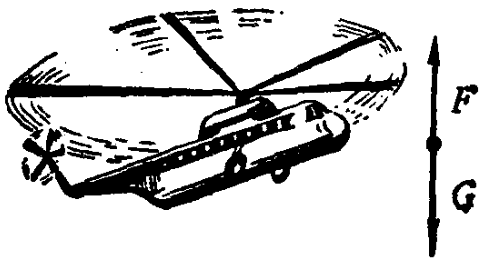
\includegraphics[width=4cm]{../pic/czwl1-ch3-8}
    \caption{}\label{fig:3-8}
\end{wrapfigure}

(1) 在地上滚动的小球,为什么越滚越慢?

(2) 机车牵引力是 $2 \times 10^5$ 牛顿,如果列车匀速行驶,它受到的阻力是多大?
如果列车的速度在增大,它受到的阻力必定小于多少?
如果列车的速度在减小,它受到的阻力必定大于多少?

(3) 重 6300 牛顿的直升飞机匀速上升或停在空中的时候(图 \ref{fig:3-8}),
螺旋桨产生的向上的举力是多大?(空气阻力不计)

(4) 用手拿住拴着钢珠的绳子,使钢珠在桌面上做曲线运动。这时,为什么手必须不断地用力牵引绳子?

